\subsection{Identification}
\label{sec:identification}
\subsubsection{Subsytem Description - Requirements}
Identification is another subsystem of the overall system. System should identify cats and feed them accordingly with a high accuracy. Identification is put just after the classification so that only cats are recognized and no more computation is required. There are different techniques in identification process such as histograms, feature descriptors, neural network based identification, and landmarks.


\begin{itemize}
    \item Identify cats with accuracy greater than 0.9.
    \item Recognize new cats and add them to database.
    \item Work in a reasonable time, aimed less than the second.
    \item Occupy space less than 1GB on the server for database.
    \item Be capable of adjust data.
    \item Advance database as more sample arrives.
\end{itemize}


\subsubsection{Explanation and Comparison of Methodology}
Every method has its own advantages and disadvantages. Comparing them and selecting the best is best explained in the following table representation. Tables \ref{tab:adv_dis_histograms}, \ref{tab:adv_dis_neural_network}, \ref{tab:adv_dis_landmarks}, and \ref{tab:adv_dis_feature_descriptors} give the comparisons for histogram, neural network, landmark, and feature descriptor based identification algorithms.

\begin{table}%[h]% This is for fine tuning at the very end
%   \begin{center}% just useless clutter
        \begin{tabularx}{\textwidth}{ X  X }\toprule
            \multicolumn{2}{c}{\textbf{\large Histogram Based Identification\strut}} \\ 
            \midrule
            \textbf{Advantages} & \textbf{Disadvantages} \\
            \midrule
            Very fast train time                    & Relatively slow identification time \\
            Easy to implement                       & Open to noise because of light, angle etc. \\
            Very powerful with different color cats & Bad performance with similar colored cats \\
            Small database requirement              & Relatively low accuracy \\
            Fast update-train time                  & Confusion as database enlarges \\
            \bottomrule
        \end{tabularx}
%   \end{center}
    \caption{Advantages and Disadvantages on the Histogram Based Identification}
    \label{tab:adv_dis_histograms}
\end{table}

\begin{table}%[h]% This is for fine tuning at the very end
%   \begin{center}% just useless clutter
        \begin{tabularx}{\textwidth}{ X  X }\toprule
            \multicolumn{2}{c}{\textbf{\large Neural Network Based Identification\strut}} \\ 
            \midrule
            \textbf{Advantages} & \textbf{Disadvantages} \\
            \midrule
            Very fast identification time           & Very slow train time \\
            Learning based, easier                  & Open to noise \\
            More powerful with more data            & Bad performance with few data \\
            Very small database requirements        & Very slow update-train time \\
                                                    & Fine-tune requirements for different environments \\
                                                    & Useless with single-shot data \\
            \bottomrule
        \end{tabularx}
%   \end{center}
    \caption{Advantages and Disadvantages on the Neural Network Based Identification}
    \label{tab:adv_dis_neural_network}
\end{table}

\begin{table}%[h]% This is for fine tuning at the very end
%   \begin{center}% just useless clutter
        \begin{tabularx}{\textwidth}{ X  X }\toprule
            \multicolumn{2}{c}{\textbf{\large Landmark Based Identification\strut}} \\ 
            \midrule
            \textbf{Advantages} & \textbf{Disadvantages} \\
            \midrule
            No train required                       & Another control of comparison required \\
            Easy to implement                       & No past experience \\
            Powerful with different kinds of cats   & Lack of train data \\
            Small database requirement              & Bigger identification time with 2-steps \\
                                                    & Very little available resources \\
            \bottomrule
        \end{tabularx}
%   \end{center}
    \caption{Advantages and Disadvantages on the Landmark Based Identification}
    \label{tab:adv_dis_landmarks}
\end{table}

\begin{table}%[h]% This is for fine tuning at the very end
%   \begin{center}% just useless clutter
        \begin{tabularx}{\textwidth}{ X  X }\toprule
            \multicolumn{2}{c}{\textbf{\large Feature Descriptor Based Identification\strut}} \\ 
            \midrule
            \textbf{Advantages} & \textbf{Disadvantages} \\
            \midrule
            Robust to illumination and angle              & Very slow train time \\
            Relatively fast identification time           & Low accuracy if no features present \\
            Powerful with detailed cats                   & Wrong matches with \\
            Useful with different environments            & \\
            Fast update-train time                        & \\
            Relatively higher performance for single shot & \\
            \bottomrule
        \end{tabularx}
%   \end{center}
    \caption{Advantages and Disadvantages on the Feature Descriptor Based Identification}
    \label{tab:adv_dis_feature_descriptors}
\end{table}

Comparison tables are self-explanatory. However some clarifications are needed. There are two train processes where train is conventional train with existing data and update-train is train for the new coming cat, image data. Neural network based identifiers require very big update-train, which is the most important drawback of them. 

\subsubsection{Data Collection and Sources}
At the end of this comparison, it should be noted that different methods have their advantages and disadvantages. Therefore, it is also possible to combine them in a way that the final decision takes considerations of different domains exhibiting different characteristics. Unfortunately, at the level of this prototype, without gathering any data, it is impossible to estimate the data behaviour in real application. What is the cat frequency, how photos are taken, what is the angle of camera, what is external lighting etc. All of these questions require answers to finish the complete fine tune of the system.

All of the systems described can be used for different environments. However, lack of data makes it really difficult to make a decision at this step when there is no working prototype present. Therefore, the most robust one is selected as it is the one which minimizes the risk, but it is pointed that there is not a single decision but a set of decisions to use different methods in accordance and assigned weights so that best results can be obtained. It should also be noted that different methods are implemented, and based on the prototype and product data, continuous switch between all of these methods are possible. More clearly, there are hyper-parameters that defines how the identification methods affect the final decision on the cat id. However, all of these adjustments and fine-tuning process is left after the prototype has been finished since no data found on the internet or another resource completely, or even nearly defines the behaviour and characteristics of data collected by the system. Finally, from now on, feature descriptors are assumed to be a generic solution to the problem. However it is always the case that a hybrid approach will be used in the actual product and the final prototype.

\subsubsection{Feature Descriptor Implementation Details}
Feature descriptors are used in identification. SIFT and ORB implementations are used and feature vectors are created for the interest points that are calculated based on known algorithms SIFT and FAST. For commercial purposes, ORB is decided to be used; however, SIFT is used in research of the product because of its slightly better performance. Note that SIFT is patented which is why ORB is going to be used in the mass production software of the product.

% sorun mu var sori bitirip bakcam
% testler cikmiyor ne yapcam ya cok uzun suruyor 2 saattir cikmadi, hmm oke
\begin{figure}[h]
    \centering
    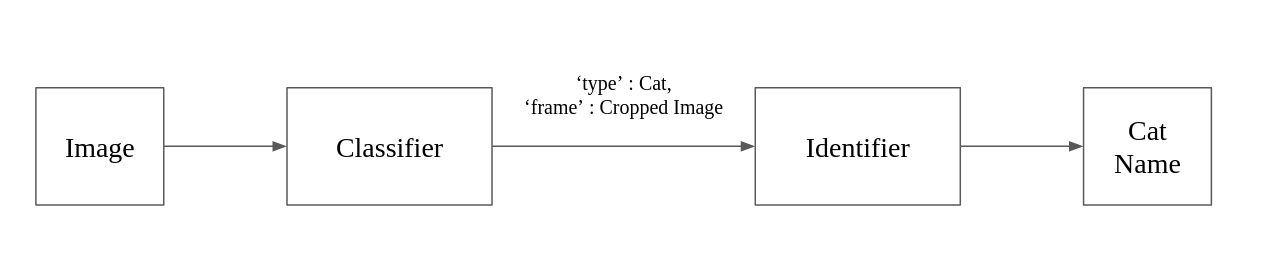
\includegraphics[width=\linewidth]{content/040_image_processing/identification/img/simpleIdentifierClassifier.png} % cok genis bu % tamamdir oyle gezerken gozume takildi kolay gelsin
    \caption{Classifier Identifier Connection}
    \label{fig:classifier_identifier_connection}
\end{figure}

% bilmiyorum ama en kotu sallayabilirsin foto falan koymadan

Identifier module requires an image with strict bound. Cropped image is directly sent to the Identifier module from Classifier module. This strict bound both prevents excessive data coming from background and smaller set of vectors to be processed. Since the angle that cats coming to eat the food is deterministic and more or less the same, background details are mostly eliminated, and an image consists only of cat head. This way, computation burden and noise are minimized.


Effect of background can be seen from figure \ref{fig:background_interest_points} and \ref{fig:iyiKedi}. Most of the features come from background. However, this image does not properly show the correct case where cats will come directly to camera. Therefore, background will lose its importance. In other words, classifier crops images in practice such that there is no background and disturbing effects. Some of the samples for this process, is given in figure \ref{fig:sampleNoBackground}. Note the Facebook database which will be explained in the next section "Test Methods and Results" consists of images with backgrounds, this is not the case thanks to the configuration of the mechanical system and classifier.

\begin{figure}
    \centering
    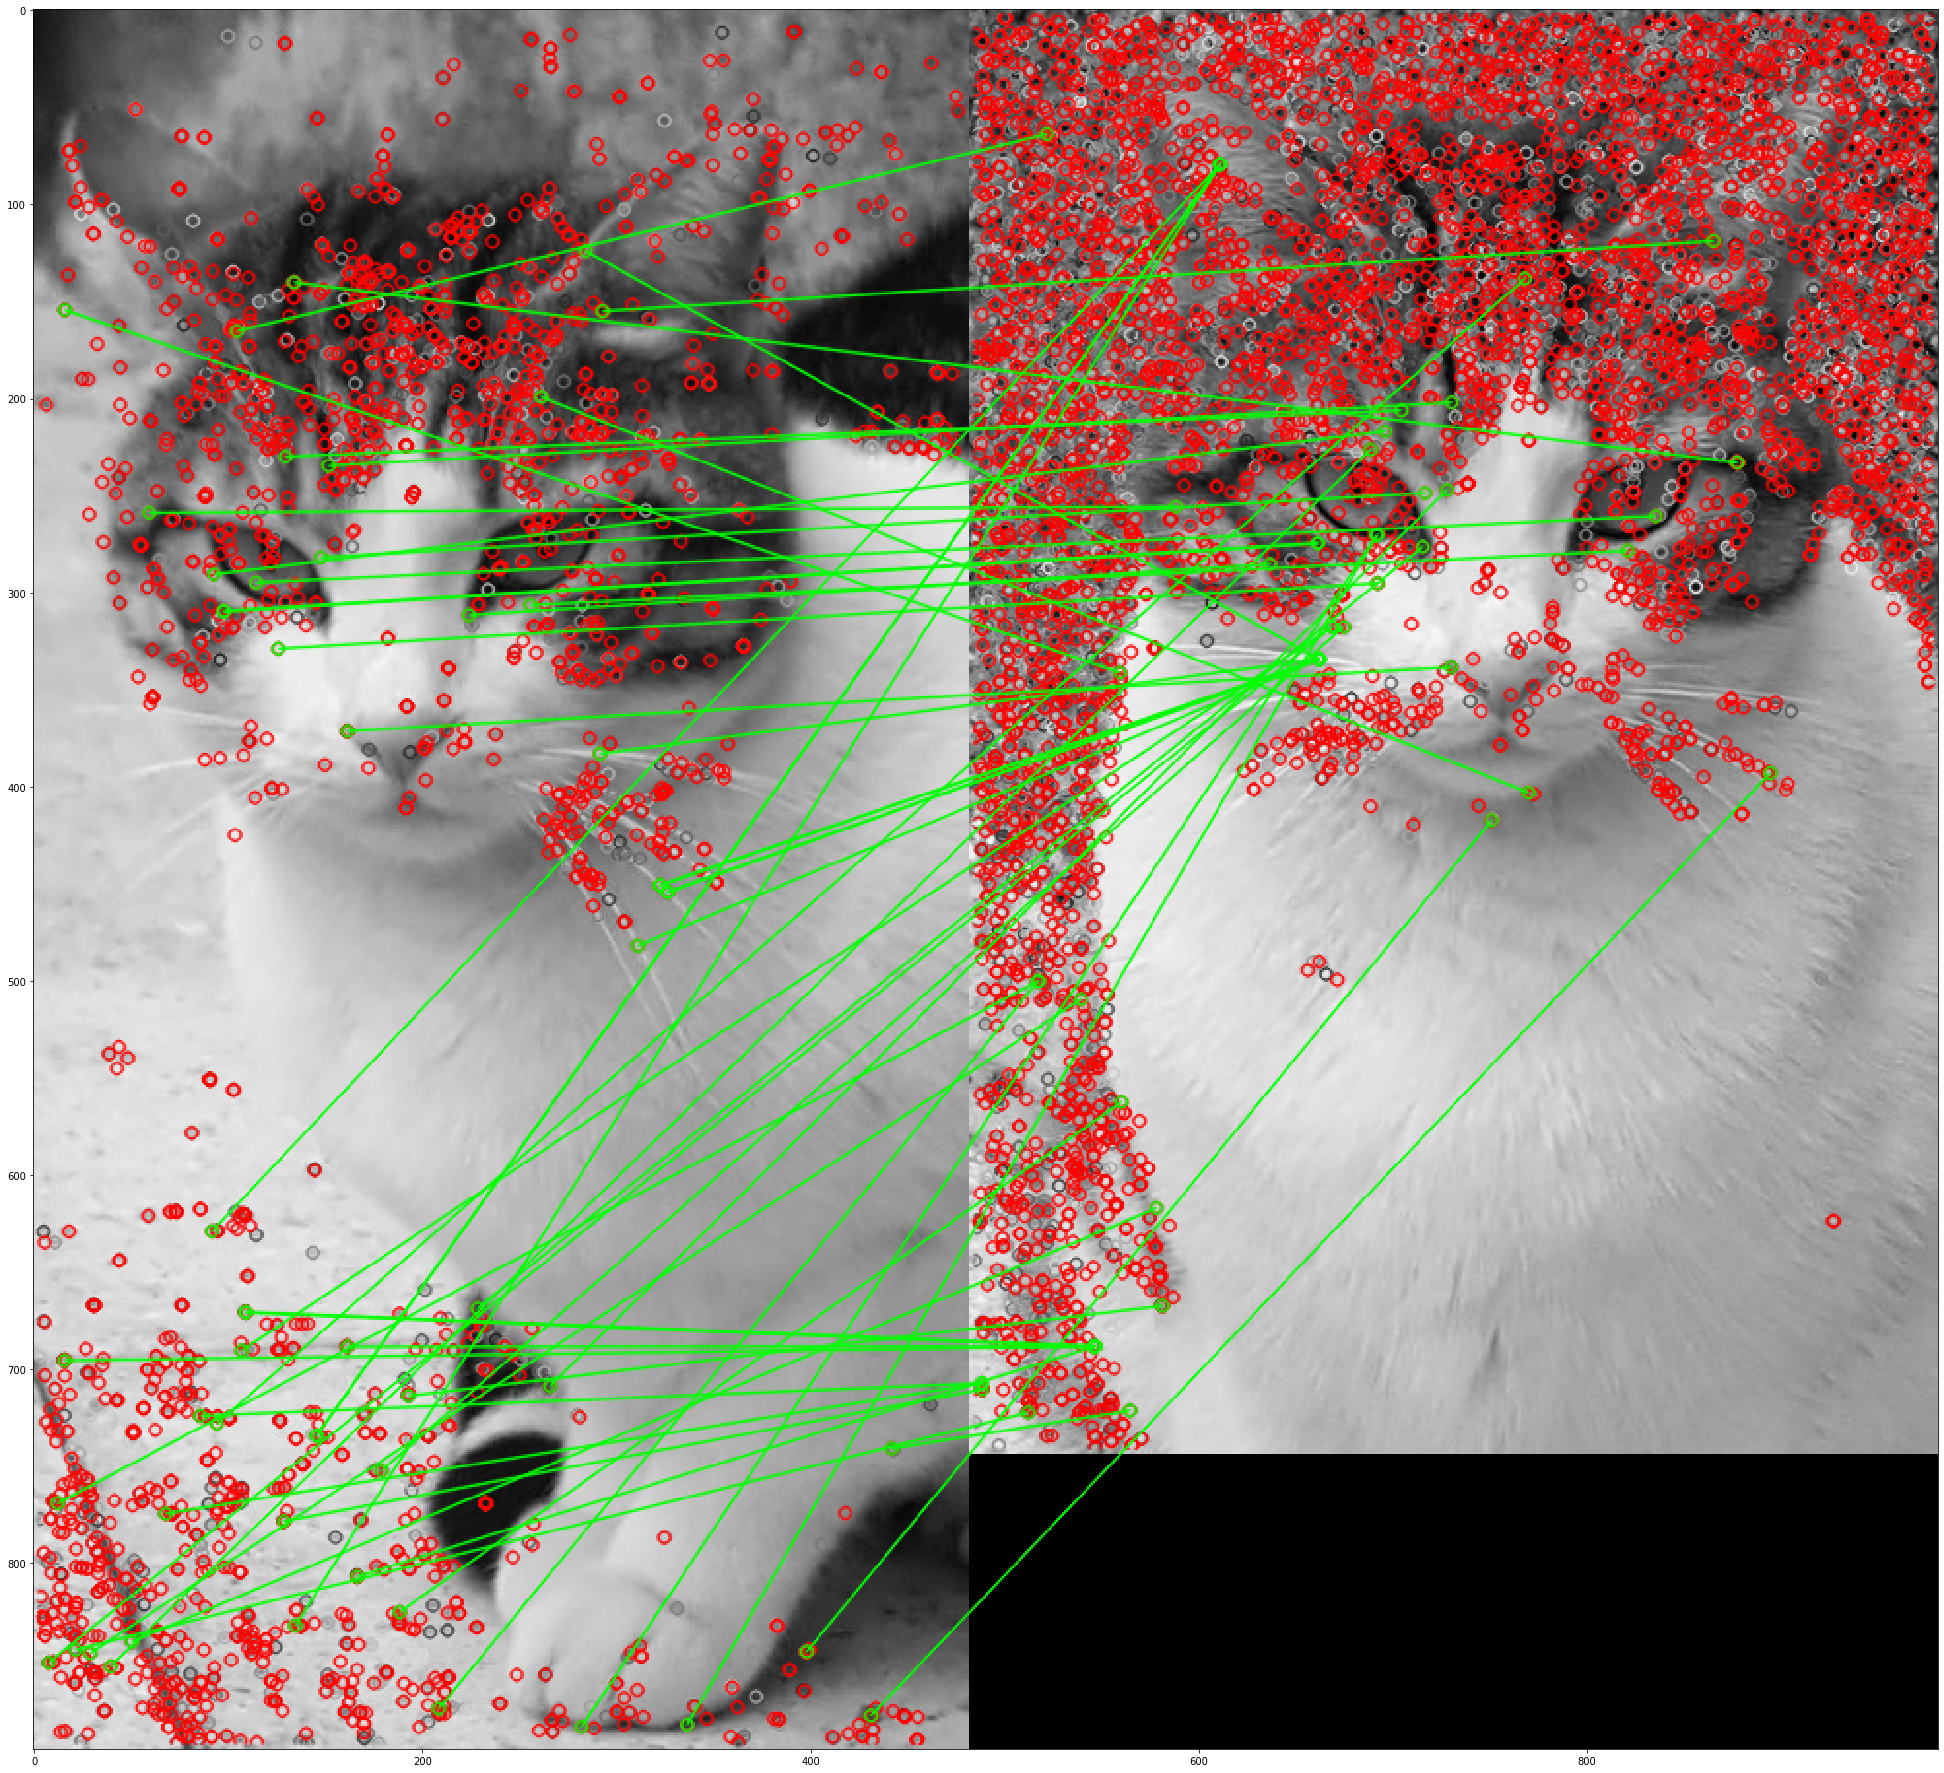
\includegraphics[width=\linewidth]{content/040_image_processing/identification/img/birsuruBackground.png}
    \caption{Background Interest Points}
    \label{fig:background_interest_points}
\end{figure}

\begin{figure}
    \centering
    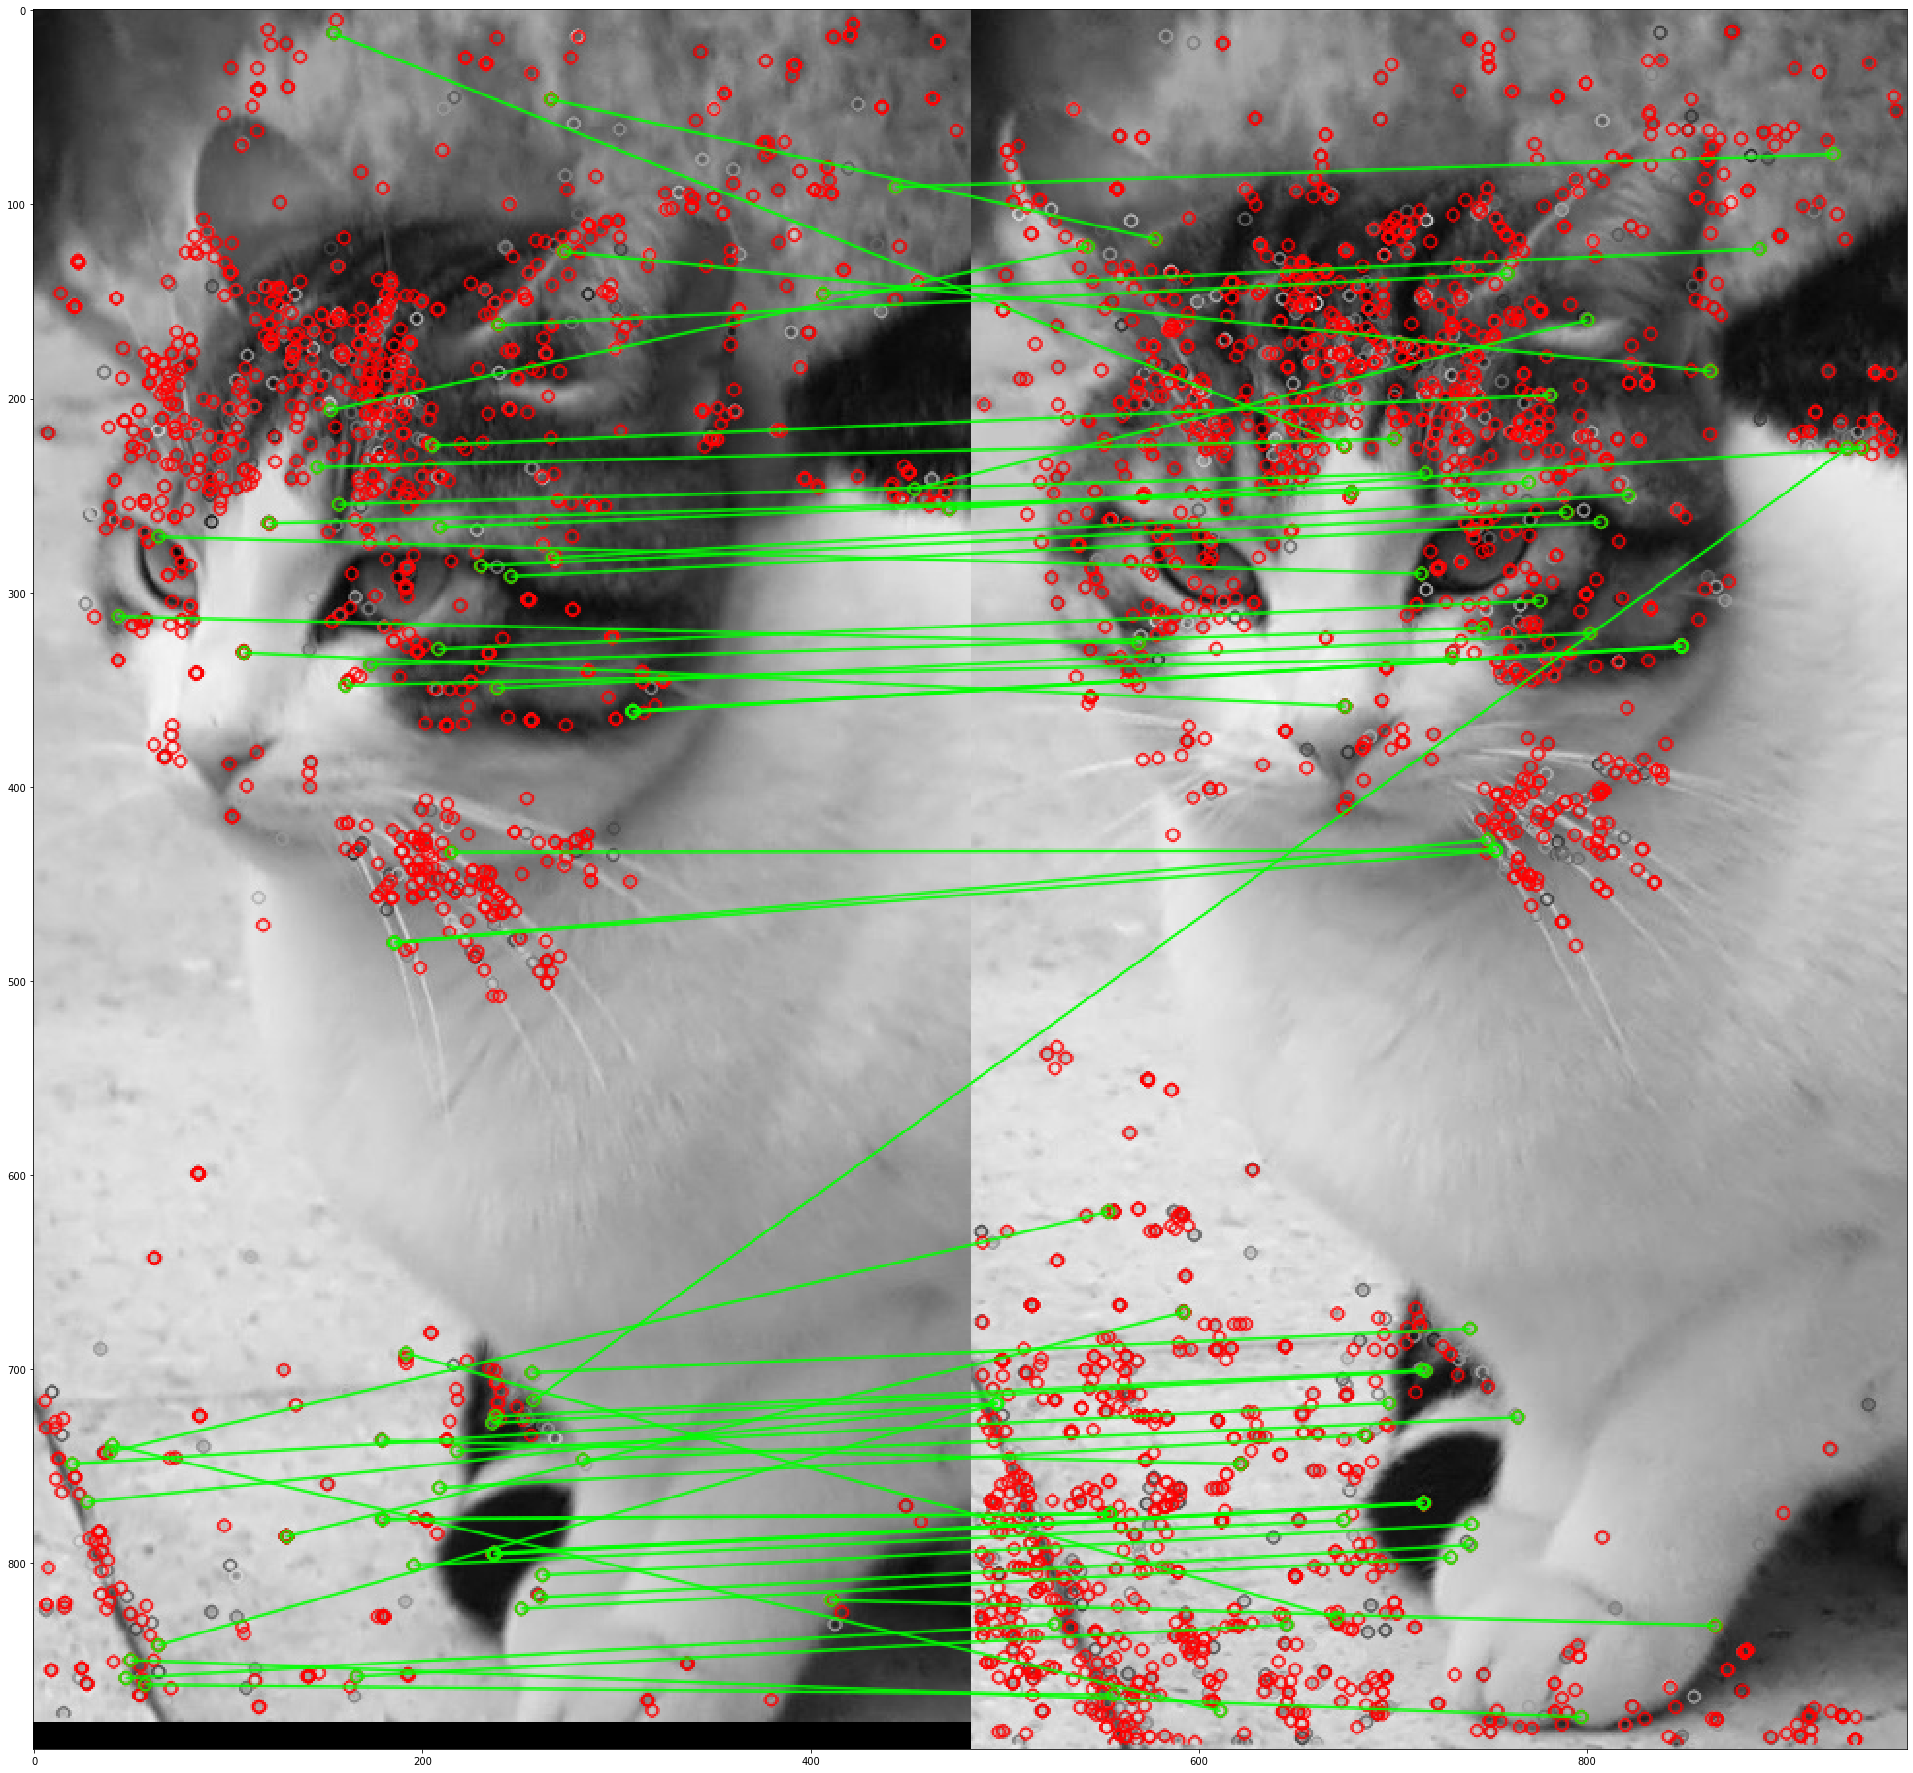
\includegraphics[width=\linewidth]{content/040_image_processing/identification/img/iyiMatchSIFTYuz.png}
    \caption{Background Match}
    \label{fig:iyiKedi}
\end{figure}

\begin{figure*}
    \centering
    \begin{subfigure}[t]{0.5\textwidth}
        \centering
        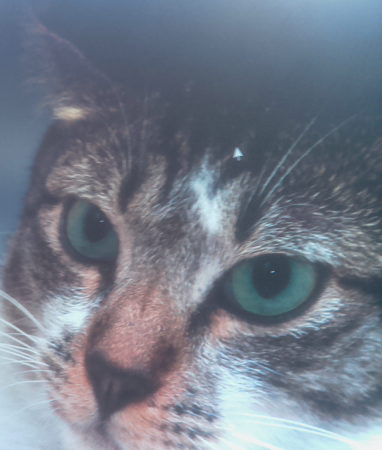
\includegraphics[height=6cm]{content/040_image_processing/identification/img/backgroundExtract1.png}
        \caption{Cat 1}
    \end{subfigure}%
    \begin{subfigure}[t]{0.5\textwidth}
        \centering
        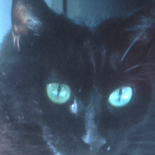
\includegraphics[height=6cm]{content/040_image_processing/identification/img/backgroundExtract2.png}
        \caption{Cat 2}
    \end{subfigure}
    \caption{Sample Images Generated by Classifier on Real Camera Shots}
    \label{fig:sampleNoBackground}
\end{figure*}



\subsubsection{Tests and Results}
It requires extra effort to make tests to determine how the sub-system does well. Both the lack of electronic and mechanical background makes it very hard to collect data directly from the camera in addition to the mobility of cats. Both finding and capturing a cat picture requires a great effort and it only allows a few sample data to be collected. Therefore, there left two possibilities; finding online cat images and using a static object. Online images are mostly consisting of random cat images that are not identified or a specific cat only appears in the pictures. Therefore, a data set is created based on the cat images shown on the computer screen and shots taken from the screen as well as Facebook group volunteers that gives samples for different cats with different names. Consequently, there exist two separate data sets, one of which is set of images for the same cat on the screen, few number of classes (cat identities), but a lot of samples, and the other one is a data set with various classes of cats but with a limited data.

3 different cat images found on the internet where neither of them is the same cat. These cat images are displayed on the computer screen and total of 100 shots were created for each cat image that is displayed. Among these 100 images there are only 60-80 possible samples which include cat, or classified correctly. Since camera gets blurry when moving and sometimes it points to different directions, it was not always possible to take pictures of cats. Therefore, only 40 - 60 sample is generated for the cat image displayed on the screen. It should be noted, to show background effect, different backgrounds, different display positions and different displays are used to display image.


Cat windows inside these images are extracted using the classification code and database created. 5 samples per class are separated for test set. Note that since there are no hyper-parameters currently optimized, there is no validation set selected and only train and test sets became in use.  
 
The other database consists of 17 different classes and 4-7 samples for each class. This is a good example of few data identification. The data set is divided to train and test sets, where test set consists of 1 sample of each class since the data is very limited. This seems a biased approach; however, system is designed for the conditions of excessively limited data. Tests are done on both data sets for different approaches and the hybrid approach at the end, and the results are given in tabular and graphical forms.

\begin{figure}
    \centering
    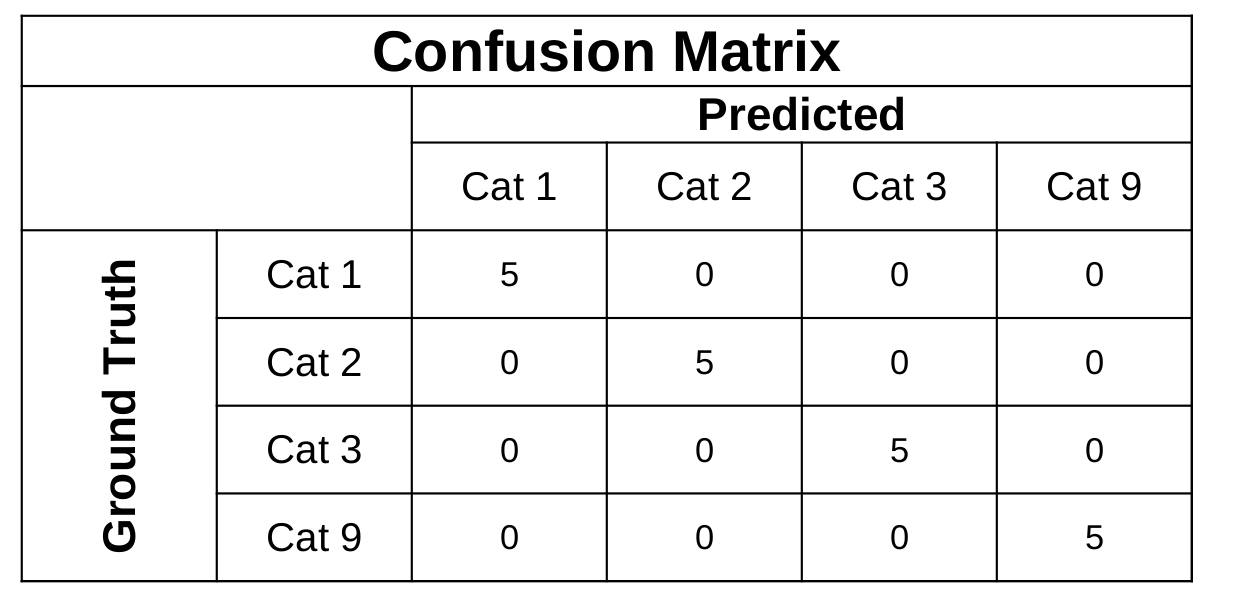
\includegraphics[width=\linewidth]{content/040_image_processing/identification/img/confusionMatrix1.png}
    \caption{Confusion Matrix for Set 1 - Test 1}
    \label{fig:confusion1}
\end{figure}

\begin{figure}
    \centering
    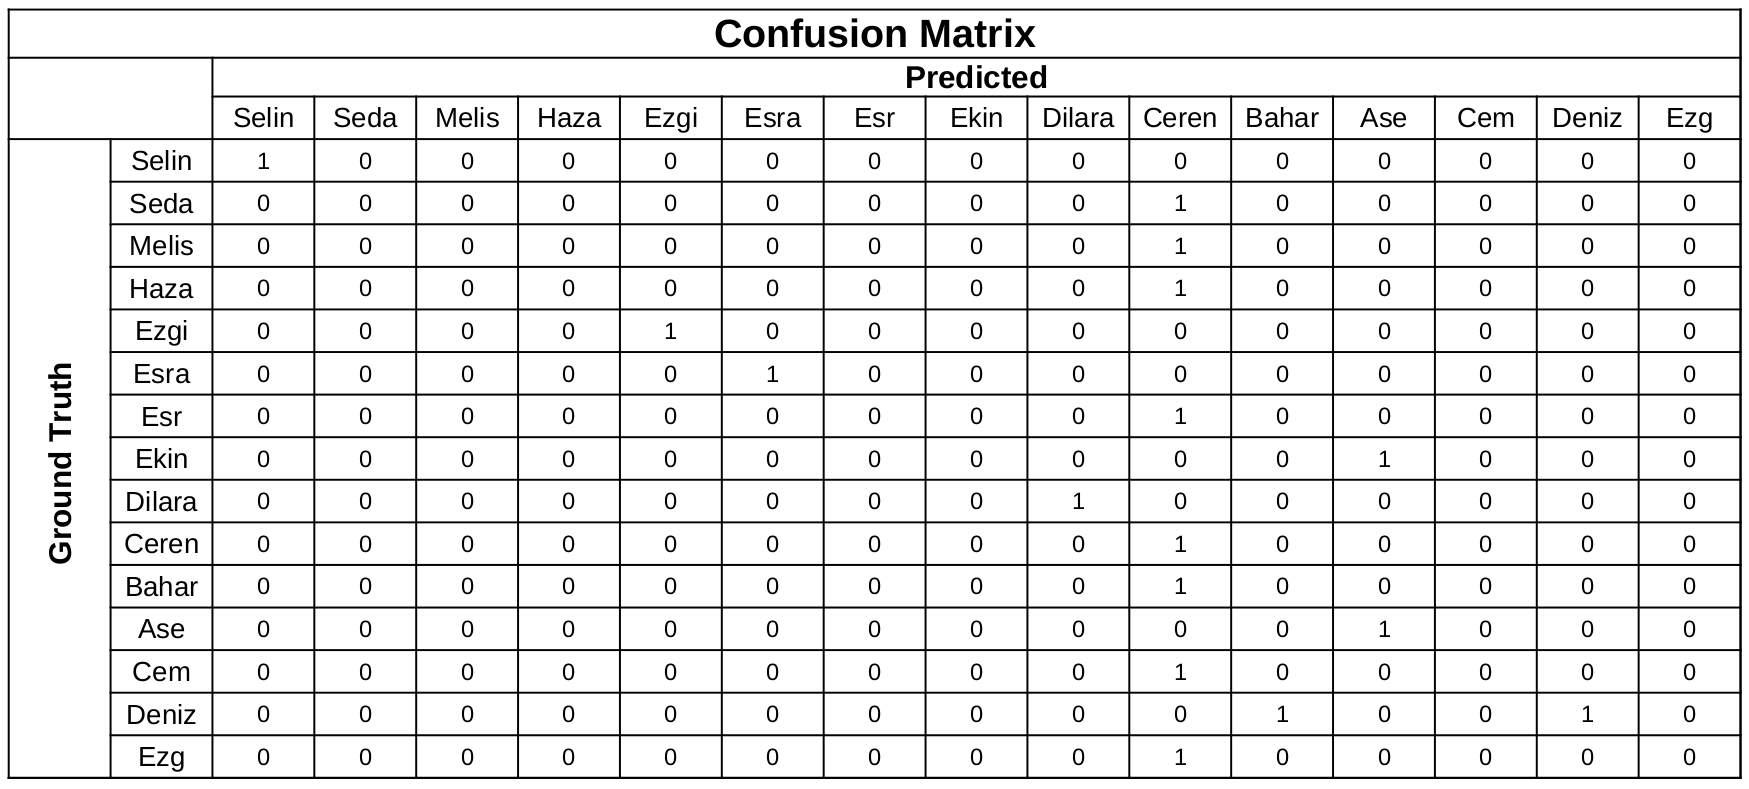
\includegraphics[width=\linewidth]{content/040_image_processing/identification/img/confusionMatrix2.png}
    \caption{Confusion Matrix for Set 2 - Test 2}
    \label{fig:confusion2}
\end{figure}

\begin{figure}
    \centering
    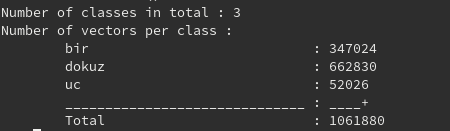
\includegraphics[width=\linewidth]{content/040_image_processing/identification/img/databaseTest2.png}
    \caption{Database Information for Test 1}
    \label{fig:databaseInfo1}
\end{figure}

\begin{figure}
    \centering
    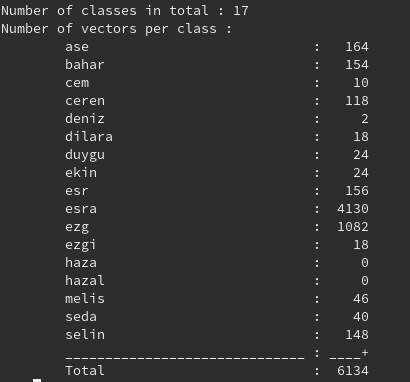
\includegraphics[width=\linewidth]{content/040_image_processing/identification/img/databaseTest3.png}
    \caption{Database Information for Test 2}
    \label{fig:databaseInfo2}
\end{figure}

\begin{figure}
    \centering
    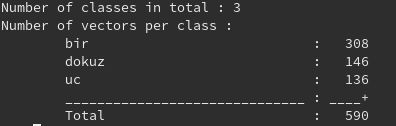
\includegraphics[width=\linewidth]{content/040_image_processing/identification/img/databaseTest4.png}
    \caption{Database Information for Test 3}
    \label{fig:databaseInfo3}
\end{figure}


\begin{figure}
    \centering
    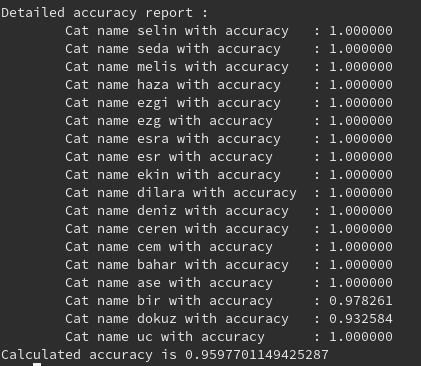
\includegraphics[width=\linewidth]{content/040_image_processing/identification/img/yeniVeriEklenince.png}
    \caption{Accuracy Tests with New Cats to the System}
    \label{fig:yeniVeriEklenince}
\end{figure}


%fatihhhhhhhhhhhhhhhhhh whatsap bak
% la cok fazla hata var en son kısımlar bitince düzeltek
% burası değişecek sal burayı tamam

There are three independent tests are done on two data sets explained above. Confusion matrix representation is given in figure \ref{fig:confusion1} and \ref{fig:confusion2} for two different data sets explained above. Moreover, technical information on database provided in figures \ref{fig:databaseInfo1} and \ref{fig:databaseInfo2} for this data sets. Note that in case of very little data, there are hardly SIFT vectors found. Test results show that, with correct camera position, and enough data accuracy can easily can go around 1.0 whereas different cameras with different angles make it to reduce even 0.3125 which is the case in figure \ref{fig:confusion2}. 


Above discussion distinguishes the behaviour on two separate sets. However, there is no single control variable to measure the actual performance. Since these data sets differ in both size and capture techniques, another data set is created which is small in train images but data collected with the same camera in different environments. This data set is tested for single shots. Single shot of a cat is taken from the camera and remaining images are put as test set. In other words, for 3 different classes, there is only 1 train sample, and 40-60 test samples. The results are astonishing in this part, accuracy is around 0.96 which is given in figure \ref{fig:yeniVeriEklenince}. In addition, new cats which are the cats the system did not see before are identified as 'None' meaning it is a new cat. The accuracy is exactly 1 which is because a threshold is dynamically adjusted for the train samples with a little loss in accuracy of the known cats, only around 0.02 - 0.07 as can be seen in figure \ref{fig:yeniVeriEklenince}.



Test results show that the system is capable of handling the cat identities with a higher accuracy. Despite the little data sources, more than 300 images and 20 classes are used in the test procedure and the results show an obvious superiority for the feature descriptors. Identification times, model train, database creation time are given below for operative perspective.

\begin{itemize}
    \item \textbf{Database creation (164 images) (54 per class) : } 6 hours 30 minutes 33 seconds
    \item \textbf{Database creation (74 images - 4.3 per class) : } 12 minutes 45 seconds 
    \item \textbf{Database creation (3 images - 1 per class)    : } 4.65 seconds
    
    \item \textbf{Image match (average) : } 0.4 seconds
\end{itemize}

The tests are done on a regular old personal computer without any acceleration or turbo technology. Single core - single thread is used in the process for better accuracy.



\begin{verbatim}
Architecture:                    x86_64
CPU op-mode(s):                  32-bit, 64-bit
Byte Order:                      Little Endian
Address sizes:                   43 bits physical, 48 bits virtual
CPU(s):                          8
On-line CPU(s) list:             0-7
Thread(s) per core:              2
Core(s) per socket:              4
Socket(s):                       1
NUMA node(s):                    1
Vendor ID:                       AuthenticAMD
CPU family:                      23
Model:                           24
Model name:                      AMD Ryzen 5 3500U 
                                 with Radeon Vega Mobile Gfx
\end{verbatim}





%% Yapılacak testler : 
% 1) Matris şeklinde her kediyi diğerleriyle karşılaştırıp accuracy veren, false positive veren tablo
% 2) Histogram şeklinde
% 3) Genel accuracy
% 4) Tepki süresi

%% Denenecek yöntemler : 
% 1) Histogram
% 2) SIFT
% 3) feature extraction
